\documentclass[cn,10pt]{OIBooks}

\title{算法竞赛模板}
\subtitle{竞赛常见代码模板}
\author{吴尧}
%\institute{Elegant\LaTeX{} Program}
\date{\today}
\version{0.1}
\bioinfo{B站}{爱学习的咸鱼君}

\extrainfo{古之立大事者,不惟有超世之才,亦必有坚忍不拔之志。—— 苏轼}

\setcounter{tocdepth}{3}

\logo{neo.jpg}
\cover{7.jpg}

% 本文档命令


\usepackage{longtable}
\usepackage{array}
%\newcommand{\ccr}[1]{\makecell{{\color{#1}\rule{1cm}{1cm}}}}

%修改标题页的橙色带
\definecolor{customcolor}{RGB}{32,178,170}
\colorlet{coverlinecolor}{customcolor}



\begin{document}

\maketitle%封面
\frontmatter
\thispagestyle{empty}
\begin{center}
  \textbf{\LARGE 文档概述}
\end{center}

\section*{排版模板参考}
\subsection*{Elegant\LaTeX{} 系列模板 \md{[核心版本]}}
ElegantLATEX 项目组致力于打造一系列美观、优雅、简便的模板方便用户使用。 目前由
ElegantNote,ElegantBook,ElegantPaper 组成,分别用于排版笔记,书籍和工作论文。
\begin{itemize}
  \item 官网:\href{https://elegantlatex.org/}{https://elegantlatex.org/}
  \item GitHub 网址:\href{https://github.com/ElegantLaTeX/}{https://github.com/ElegantLaTeX/}
\end{itemize}
\section*{书籍内容参考}
\subsection*{《算法竞赛》 \md{[罗勇军]}}
本书是一本全面、深入解析与算法竞赛有关的数据结构、算法、代码的计算机教材

本书包括十个专题: 基础数据结构、基本算法、搜索、高级数据结构、动态规划、数论和线性代数、组合数学、计算几何、字符串和图论。本书覆盖了绝大多数算法竞赛考点。

本书解析了算法竞赛考核的数据结构、算法; 组织了每个知识点的理论解析和经典例题; 给出了简洁、精要的模板代码; 通过明快清晰的文字、透彻的图解,实现了较好的易读性。

本书的读者对象是参加算法竞赛的中学生和大学生、准备面试IT企业算法题的求职者、需要提高算法能力的开发人员,以及对计算机算法有兴趣的广大科技工作者。
\subsection*{《深入浅出程序设计竞赛 基础篇》 \md{[汪楚奇]}}
本书分为4部分:第1部分介绍C++语言的基础知识,包括表达式、变量、分支、循环、数组、函数、字符串、结构体等内容;第2部分介绍一些基础算法,包括模拟、高精度、排序、枚举、递推、递归、贪心、二分、搜索等;第3部分介绍几种简单常用的数据结构,包括线性表、二叉树、并查集、哈希表和图;第4部分是在算法竞赛中需要使用的数学基础,包括位运算与进制转换、计数原理、排列与组合、质数与合数、约数与倍数等概念。

本书主要面向从未接触过程序设计竞赛(包括NOI系列比赛、ICPC系列比赛)的选手,也适用于稍有接触算法、希望进一步巩固算法基础的读者。

本书提供一些在线的配套资源,例如课件或勘误表,读者可以发邮件至编辑邮箱1548103297@qq.com索取。
\subsection*{《深入浅出程序设计竞赛 进阶篇》\md{[汪楚奇]}}
该书未出版,可通过购买洛谷月赛年卡,以课程赠品的形式获得书稿。

本书分为5部分:第1部分介绍 进阶技巧与思想,包括常见优化技巧、前缀和、差分与离散化、分治与倍增等内容;第2部分介绍一些进阶数据结构,包括二叉堆与树状数组、线段树、字符串等内容;第3部分介绍图论相关算法,包括树、最短路、最小生成树、连通性等内容;第4部分介绍动态规划相关知识,包括线性动态规划、区间与环形动态规划、树与图上的动态规划等内容;第5部分介绍数学,包括进阶数论、组合数学与计算、概率与统计等内容。

\subsection*{《算法竞赛入门经典》 \md{[刘汝佳]}}
《算法竞赛入门经典(第2版)》是一本算法竞赛的入门与提高教材,把C/C++语言、算法和解题有机地结合在一起,淡化理论,注重学习方法和实践技巧。全书内容分为12章,包括程序设计入门、循环结构程序设计、数组和字符串、函数和递归、C++与STL入门、数据结构基础、暴力求解法、高效算法设计、动态规划初步、数学概念与方法、图论模型与算法、高级专题等内容,覆盖了算法竞赛入门和提高所需的主要知识点,并含有大量例题和习题。书中的代码规范、简洁、易懂,不仅能帮助读者理解算法原理,还能教会读者很多实用的编程技巧;书中包含的各种开发、测试和调试技巧也是传统的语言、算法类书籍中难以见到的。

《算法竞赛入门经典(第2版)》可作为全国青少年信息学奥林匹克联赛(NOIP)复赛教材、全国青少年信息学奥林匹克竞赛(NOI)和ACM国际大学生程序设计竞赛(ACM/ICPC)的训练资料。
\subsection*{《算法竞赛进阶指南》 \md{[李煜东]}}


本书主要根据CCF-NOI信息学奥林匹克竞赛涉及的知识体系进行编写,对计算机程序设计的基本技能——数据结构与算法进行了深入的讲解。

本书面向已经掌握至少一门程序设计语言、对于算法设计有入门性认识的读者,以各类知识点之间的贯穿联系为主线,通过各种模型与例题对各种思维方向进行深入引导,让读者在阅读本书后对算法设计初步具有整体掌控性的理解。能够让读者由浅入深地体会算法,学习算法。

本书融合了作者在算法设计教育领域、算法竞赛参赛与指导领域10年来的一线经验,其特色是训练读者算法设计的思维习惯,而非对知识流水的记忆性诵读,能让认真阅读本书并完成所有练习的读者,逐渐具有NOIP竞赛一等奖以上的实力。

\subsection*{《算法训练营 进阶篇》\md{[陈小玉]}}
《算法训练营:海量图解+竞赛刷题(进阶篇)》以海量图解的形式,详细讲解常用的数据结构与算法,并结合竞赛实例引导读者进行刷题实战。通过对本书的学习,读者可掌握22种高级数据结构、7种动态规划算法、5种动态规划优化技巧,以及5种网络流算法,并熟练应用各种算法解决实际问题。

%\newpage
\frontmatter
\thispagestyle{empty}

\begin{longtable}{m{3cm}<{\centering}m{5cm}<{\centering}m{3cm}<{\centering}}
	\caption*{{\LARGE 致谢名单}} \\ \toprule
	编号 & 昵称  & 打赏 \\ \midrule
	null & null & null  \\
	null & null & null \\ 
	\bottomrule
\end{longtable}



\begin{center}	
	如果你喜欢本文档,欢迎打赏! \\[1pt]
	\begin{figure}[H]
		\begin{minipage}[t]{0.5\linewidth}
			\centering
			
\includegraphics[width=.5\linewidth]{00chapter/wxpng}
			\caption{微信打赏}
		\end{minipage}
		\begin{minipage}[t]{0.5\linewidth}
		\centering
		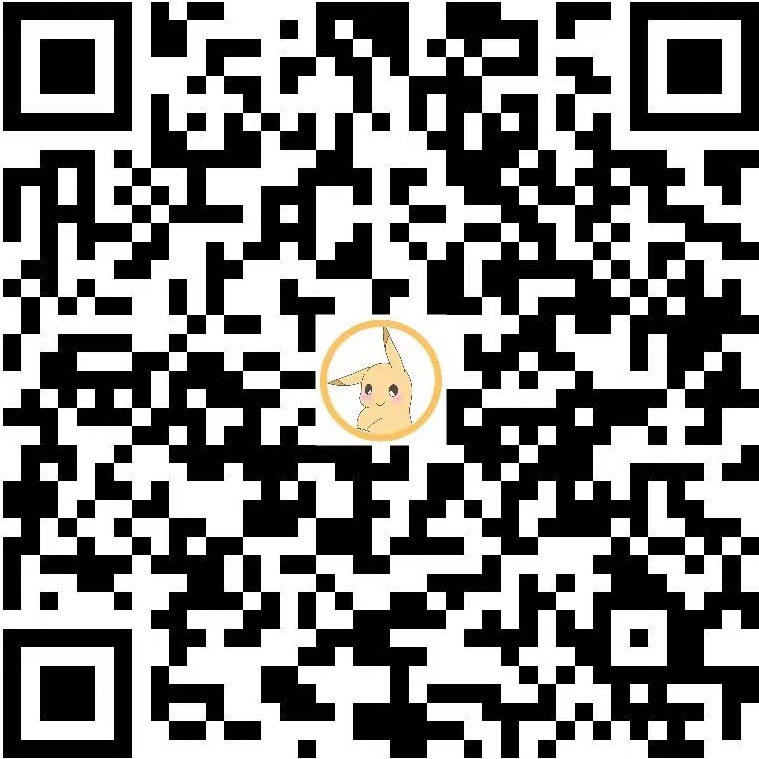
\includegraphics[width=.5\linewidth]{00chapter/zfbpng}
		\caption{支付宝打赏}
		\end{minipage}	
	\end{figure}
\end{center}

\tableofcontents%目录

\mainmatter
\part{C++程序设计}
\chapter{程序基本语句}
\section{默认框架}
\begin{lstlisting}[style=cpp]
#include <bits/stdc++.h>  //万能头,基本包含所需的头文件
using namespace std;
using i64 = long long;  // 使用i64作为long long类型的别名
const int N = 1e5 + 5;  // 范围常量 N
int main() {
	ios::sync_with_stdio(false);  // 关闭同步流,加速输入输出
	cin.tie(nullptr);
	
	return 0;
}
\end{lstlisting}

\section{快读}



%默认框架
\chapter{基础程序与输出}
\section{第一个程序}

\begin{problemset}
\item 洛谷B2002 Hello,World!
\item 洛谷B2025 输出字符菱形
\item 洛谷P1000 超级玛丽游戏
\end{problemset}


%

\part{数据结构}
\chapter{线性表}
\section{双端栈}
\section{优先队列}
\section{倍增(ST表)}


\begin{problemset}
\item 洛谷B2002 Hello,World!
\item 洛谷B2025 输出字符菱形
\item 洛谷P1000 超级玛丽游戏
\end{problemset}


%线性表
\chapter{线性结构}
\section{双端栈}
\section{优先队列}
\section{倍增(ST表)}


\begin{problemset}
\item 洛谷B2002 Hello,World!
\item 洛谷B2025 输出字符菱形
\item 洛谷P1000 超级玛丽游戏
\end{problemset}


%线性结构
\chapter{序列}
\section{跳跃表}



\begin{problemset}
\item 洛谷B2002 Hello,World!
\item 洛谷B2025 输出字符菱形
\item 洛谷P1000 超级玛丽游戏
\end{problemset}


%序列
\chapter{简单树}
\section{二叉树的遍历}



\begin{problemset}
\item 洛谷B2002 Hello,World!
\item 洛谷B2025 输出字符菱形
\item 洛谷P1000 超级玛丽游戏
\end{problemset}


%简单树
\chapter{复杂树}
\section{树链剖分}



\begin{problemset}
\item 洛谷B2002 Hello,World!
\item 洛谷B2025 输出字符菱形
\item 洛谷P1000 超级玛丽游戏
\end{problemset}


%复杂树
\chapter{集合与森林}
\section{并查集}



\begin{problemset}
\item 洛谷B2002 Hello,World!
\item 洛谷B2025 输出字符菱形
\item 洛谷P1000 超级玛丽游戏
\end{problemset}


%集合与森林
\chapter{特殊树}
\section{线段树}

\begin{problemset}
\item 洛谷B2002 Hello,World!
\item 洛谷B2025 输出字符菱形
\item 洛谷P1000 超级玛丽游戏
\end{problemset}

\section{字典树}
\begin{pro}
	
洛谷 P8306 字典树 

\url{https://www.luogu.com.cn/problem/P8306}
\end{pro}

\begin{lstlisting}[style=cpp]
#include <bits/stdc++.h>
using namespace std;
using i64 = long long;
const int N = 1e5 + 5;
const int M = 3e6 + 5;
int toNum[256];  // toNum[字符]=数字(分支位置)
struct node {
	int son[65];  // 分支 每个字母对应一个
	int num;      // 树根到该节点的前缀出现次数
	bool end;     // 是否是单词的结尾
} trie[M];
int tot;  // 字典树节点个数,trie[0]为根节点
void init() {
	for (int i = 0; i < 26; i++) {
		toNum[i + 'a'] = i;
		toNum[i + 'A'] = i + 26;
	}
	for (int i = 0; i < 10; i++) {
		toNum[i + '0'] = i + 52;
	}
}
void insert(string s) {
	int len = s.size();
	int u = 0;
	for (int i = 0; i < len; i++) {
		int ch = toNum[(int)s[i]];
		if (!trie[u].son[ch])  // 当前分支第一次出现
		trie[u].son[ch] = ++tot;  // 将tot分配给新分支的字母ch,记录对应位置
		u = trie[u].son[ch];  // 更新位置
		trie[u].num++;        // 更新前缀单词个数
	}
	trie[u].end = 1;  // 标记结尾
}
int findPre(string s) {
	int len = s.size();
	int u = 0;
	for (int i = 0; i < len; i++) {
		int ch = toNum[(int)s[i]];
		if (!trie[u].son[ch]) return 0;  // 字符串s不存在
		u = trie[u].son[ch];             // 更新位置
	}
	return trie[u].num;  // 返回前缀s的个数
}
int main() {
	ios::sync_with_stdio(false);
	cin.tie(nullptr);
	int n, q, t;
	string s;
	init();
	cin >> t;
	while (t--) {
		for (int i = 0; i <= tot; i++) trie[i] = {0};
		tot = 0;
		cin >> n >> q;
		for (int i = 1; i <= n; i++) {
			cin >> s;
			insert(s);
		}
		for (int i = 1; i <= q; i++) {
			cin >> s;
			cout << findPre(s) << '\n';
		}
	}
	return 0;
}	
\end{lstlisting}

\begin{problemset}
	\item 洛谷B2002 Hello,World!
	\item 洛谷B2025 输出字符菱形
	\item 洛谷P1000 超级玛丽游戏
\end{problemset}

%特殊树

\part{算法}
\chapter{基础算法}
\section{二分法}
\section{倍增法}
\section{分治法}


\begin{problemset}
\item 洛谷B2002 Hello,World!
\item 洛谷B2025 输出字符菱形
\item 洛谷P1000 超级玛丽游戏
\end{problemset}


%基础算法
\chapter{数值处理算法}
\section{高精度加法}
\section{高精度减法}
\section{高精度乘法}

\section{高精度整数除以低精度整数}

\begin{problemset}
\item 洛谷B2002 Hello,World!
\item 洛谷B2025 输出字符菱形
\item 洛谷P1000 超级玛丽游戏
\end{problemset}


%数值处理算法
\chapter{排序算法}
\section{冒泡排序}
\section{简单选择排序}
\section{简单插入排序}

\section{归并排序}

\section{快速排序}

\begin{problemset}
\item 洛谷B2002 Hello,World!
\item 洛谷B2025 输出字符菱形
\item 洛谷P1000 超级玛丽游戏
\end{problemset}


%排序算法
\chapter{基础算法}
\section{二分法}
\section{倍增法}
\section{分治法}


\begin{problemset}
\item 洛谷B2002 Hello,World!
\item 洛谷B2025 输出字符菱形
\item 洛谷P1000 超级玛丽游戏
\end{problemset}


%搜索算法
\chapter{数值处理算法}
\section{高精度加法}
\section{高精度减法}
\section{高精度乘法}

\section{高精度整数除以低精度整数}

\begin{problemset}
\item 洛谷B2002 Hello,World!
\item 洛谷B2025 输出字符菱形
\item 洛谷P1000 超级玛丽游戏
\end{problemset}


%图论算法
\chapter{排序算法}
\section{冒泡排序}
\section{简单选择排序}
\section{简单插入排序}

\section{归并排序}

\section{快速排序}

\begin{problemset}
\item 洛谷B2002 Hello,World!
\item 洛谷B2025 输出字符菱形
\item 洛谷P1000 超级玛丽游戏
\end{problemset}


%动态规划算法
\chapter{排序算法}
\section{冒泡排序}
\section{简单选择排序}
\section{简单插入排序}

\section{归并排序}

\section{快速排序}

\begin{problemset}
\item 洛谷B2002 Hello,World!
\item 洛谷B2025 输出字符菱形
\item 洛谷P1000 超级玛丽游戏
\end{problemset}


%字符串相关算法

\part{数学}
\chapter{初等数论}

\section{欧几里得算法}

\begin{problemset}
	\item 洛谷B2002 Hello,World!
	\item 洛谷B2025 输出字符菱形
	\item 洛谷P1000 超级玛丽游戏
\end{problemset}

\section{拓展欧几里得}

\begin{problemset}
	\item 洛谷B2002 Hello,World!
	\item 洛谷B2025 输出字符菱形
	\item 洛谷P1000 超级玛丽游戏
\end{problemset}

\section{质数筛法}


\subsection{埃氏筛}



\subsection{欧拉筛}


\begin{problemset}
\item 洛谷B2002 Hello,World!
\item 洛谷B2025 输出字符菱形
\item 洛谷P1000 超级玛丽游戏
\end{problemset}




%\printbibliography[heading=bibintoc, title=\ebibname]
\appendix
\chapter{VS Code安装与C++环境配置}
\begin{introduction}
	\item 计算机选购
	\item 操作系统
	\item \texttt{IDE}安装
	\item 网站推荐
	\item 学习方法
	\item 学习心态
\end{introduction}

俗话说三军未动,粮草先行。在正式开启信奥的学习之前,我们先把准备工作做好。
\section{安装g++编译器}

\section{安装VS Code}

\section{配置C++环境}




\chapter{NOI Linux 2.0系统情况简表}
% Please add the following required packages to your document preamble:
% \usepackage{multirow}
\begin{table}[H]
	\begin{tabular}{|l|l|l|l|}
		\hline
		类别                      & 软件/模块                   & 版本             & 备注说明                    \\ \hline
		系统                      & Kernel                  & 5.4-42-generic & 64位                     \\ \hline
		\multirow{5}{*}{语言环境}   & GCC                     & 9.3.0          & C编译器                    \\ \cline{2-4} 
		& G++                     & 9.3.0          & C++编译器                  \\ \cline{2-4} 
		& FPC                     & 3.0.4          & Pascal编译器               \\ \cline{2-4} 
		& \multirow{2}{*}{Python} & 2.7            & 非竞赛语言                   \\ \cline{3-4} 
		&                         & 3.8            & 非竞赛语言                   \\ \hline
		\multirow{2}{*}{调试工具}   & GDB                     & 9.1            &                         \\ \cline{2-4} 
		& DDD                     & 3.3.12         &                         \\ \hline
		\multirow{3}{*}{集成开发环境} & Code::Blocks            & 20.03          & C/C++集成开发环境             \\ \cline{2-4} 
		& Lazarus                 & 2.0.6          & Pascal集成开发环境            \\ \cline{2-4} 
		& Geany                   & 1.36           & C/C++/Pascal(轻量级)集成开发环境 \\ \hline
		\multirow{7}{*}{文本编辑工具} & VS Code                 & 1.54.3         &                         \\ \cline{2-4} 
		& Emacs                   & 26.3           &                         \\ \cline{2-4} 
		& Gedit                   & 3.36.2         &                         \\ \cline{2-4} 
		& Vim                     & 8.1            &                         \\ \cline{2-4} 
		& Joe                     & 4.6            &                         \\ \cline{2-4} 
		& nano                    & 4.8            &                         \\ \cline{2-4} 
		& sublime text            & 3.2.2          &                         \\ \hline
		\multirow{4}{*}{其他软件}   & Firefox                 & 79.0           & 网页浏览器                   \\ \cline{2-4} 
		& Midnight Commander(mc)  & 4.8.24         & 终端                      \\ \cline{2-4} 
		& Xterm(UXTerm)           & 3.5.3          & 终端                      \\ \cline{2-4} 
		& Arbiter-local           & 1.02           & 程序测评工具单机版               \\ \hline
	\end{tabular}
\end{table}




\end{document}
